\documentclass{article}
\usepackage[utf8]{inputenc}
\usepackage{geometry}
\usepackage{graphicx}
\usepackage{hyperref}

\geometry{
left=25mm,
right=25mm,
top=20mm,
bottom=25mm
}

\title{\textbf{Report N° MSc Thesis: Active Constraints}}
\author{\textbf{Alberto Rota} - \textit{Supervisor: Prof. Elena De Momi}}
\date{}

\begin{document}
\maketitle
\paragraph{Title:} \textit{To Be Defined}
\section*{General guidelines}
    Development of surgical training tasks implementing Active Constraints of
    different nature and with different levels of intervention, in order to
    evaluate their efficacy and role in Robot-Assisted Minimally Invasive Sugery.
    \begin{itemize}
        \item \textit{Phase 1: }Software Development in a virtual environment (Unity)
        \item \textit{Phase 2: }Implementing on the dVRK, followed by
        experimental tests with data gathering, analysis and validation
    \end{itemize}
\section*{Progress}
    
\section*{Next Steps}
    
\newpage
\section*{Screenshots}
% \begin{figure}[h!]
%     \begin{small}
%         \begin{center}
%             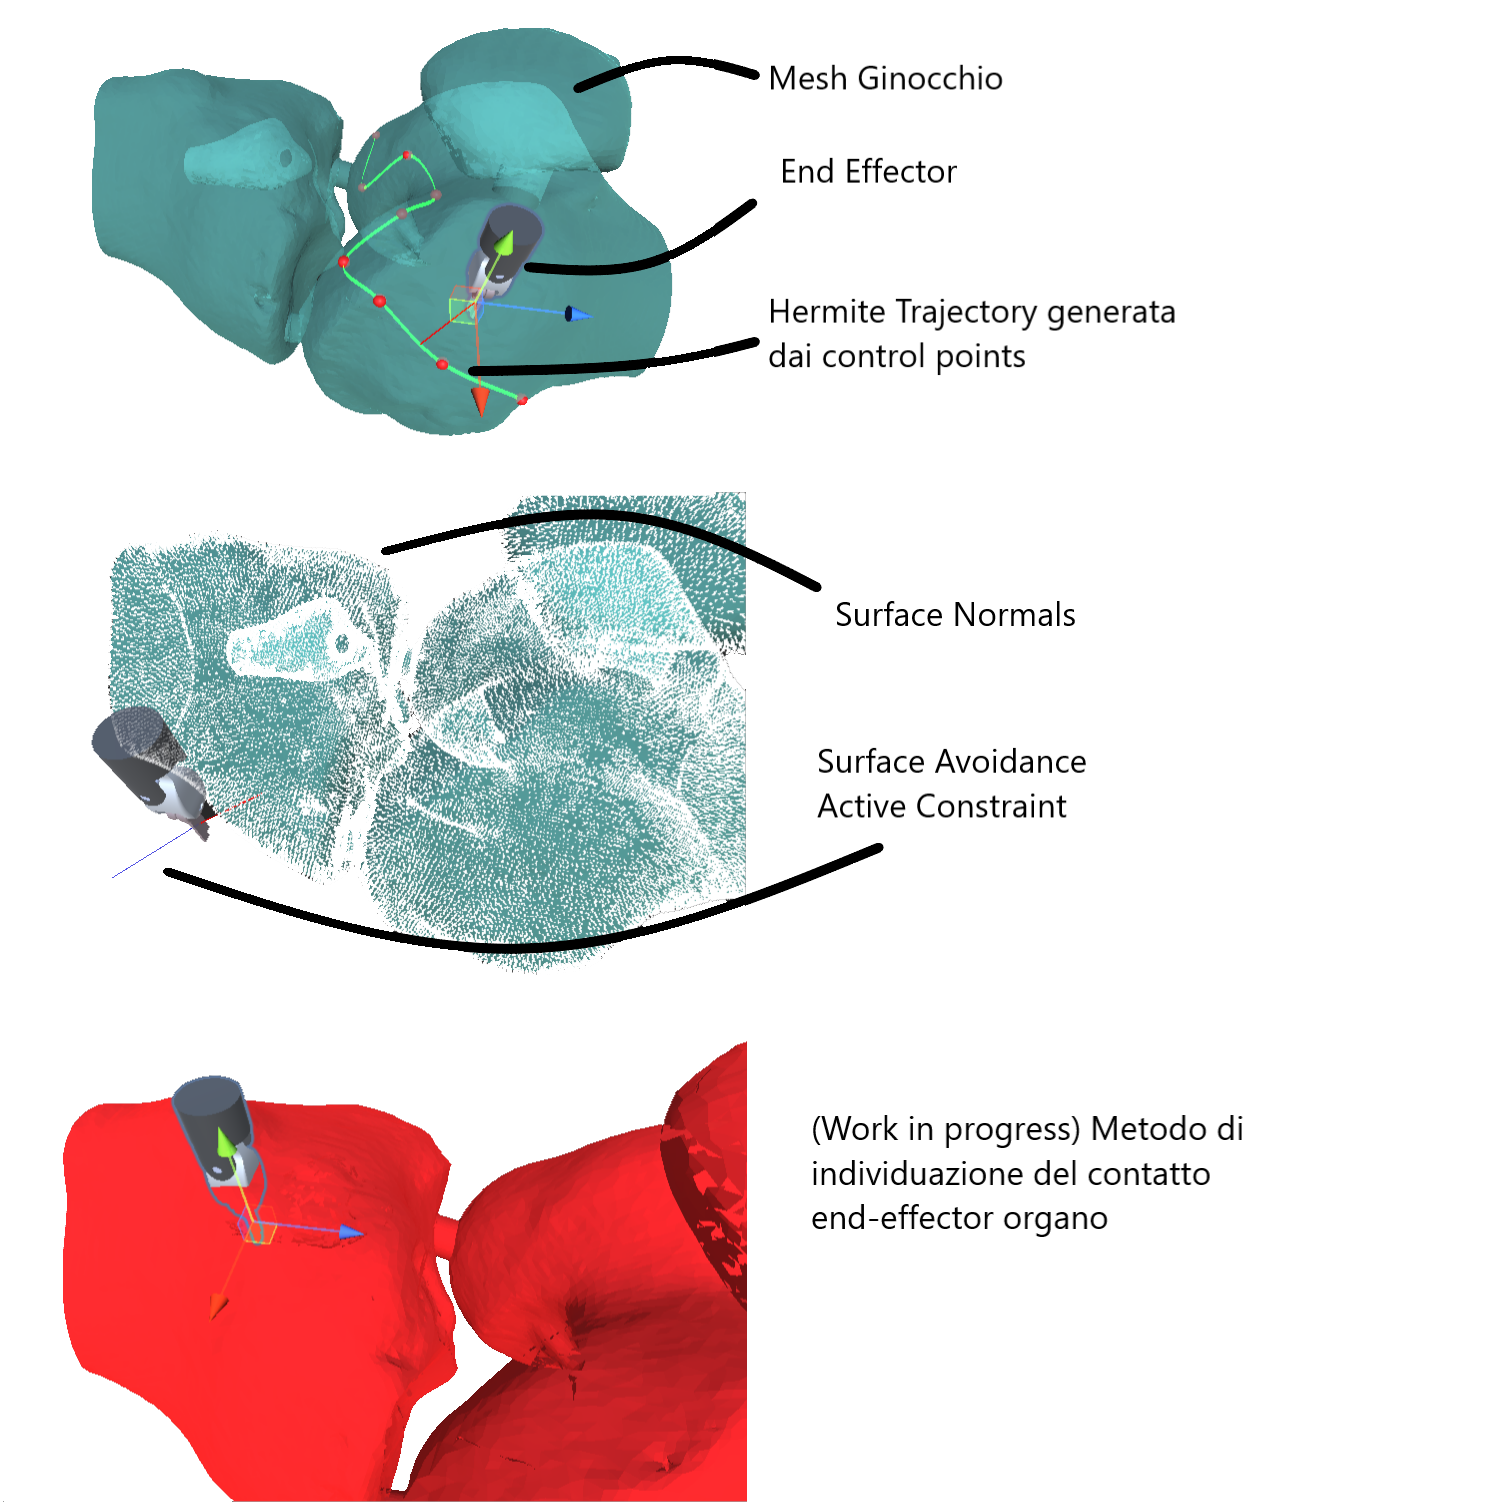
\includegraphics[width=0.95\textwidth]{Scene.png}
%         \end{center}
%         \label{fig:}
%     \end{small}
% \end{figure}

    
\end{document}